% Created 2022-09-19 Mon 16:19
\documentclass[9pt, b5paaper]{book}
\usepackage{xeCJK}
\usepackage[T1]{fontenc}
\usepackage[scaled]{beraserif}
\usepackage[scaled]{berasans}
\usepackage[scaled]{beramono}
\usepackage{graphicx}
\usepackage{xcolor}
\usepackage{multirow}
\usepackage{multicol}
\usepackage{float}
\usepackage{textcomp}
\usepackage{geometry}
\geometry{left=1.2cm,right=1.2cm,top=1.5cm,bottom=1.2cm}
\usepackage{algorithm}
\usepackage{algorithmic}
\usepackage{latexsym}
\usepackage{natbib}
\usepackage{minted}
\newminted{common-lisp}{fontsize=\footnotesize}
\usepackage[xetex,colorlinks=true,CJKbookmarks=true,linkcolor=blue,urlcolor=blue,menucolor=blue]{hyperref}
\author{Heyan Jenny Huang}
\date{\today}
\title{Appellant's Desigtnation of Record on Appeal}
\hypersetup{
  pdfkeywords={},
  pdfsubject={},
  pdfcreator={Emacs 27.1 (Org mode 8.2.7c)}}
\begin{document}

\maketitle
\tableofcontents


\chapter{几个主要的关注点:根据表哥的陈述,每条反驳回去}
\label{sec-1}
\begin{itemize}
\item to be summarized and finished this evening
\end{itemize}
\section{现有的案件}
\label{sec-1-1}

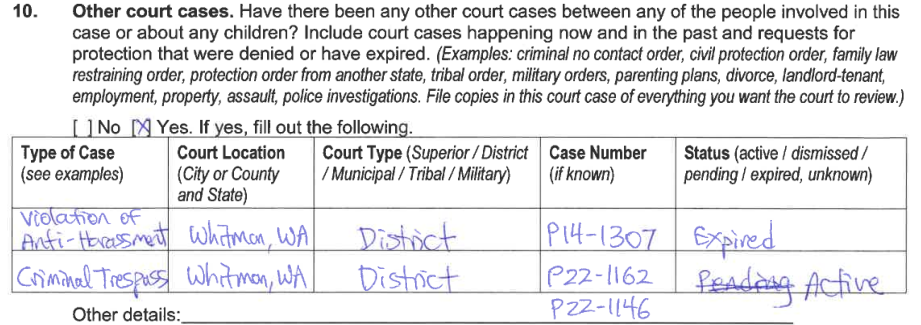
\includegraphics[width=.9\linewidth]{./pic/dearCousin_20220919_153339.png}
\begin{itemize}
\item 是当地的法院没有及时地通知我或是办理案件,让我没有机会学习和校正自己的行为, 不管是6/17号的,还是接下来的,我没有机会学习来校正自己
\end{itemize}
\section{保护令的时长,一年,多于一年,一辈子(法官真是生猛呀,一令就是一辈子。。。。。)}
\label{sec-1-2}

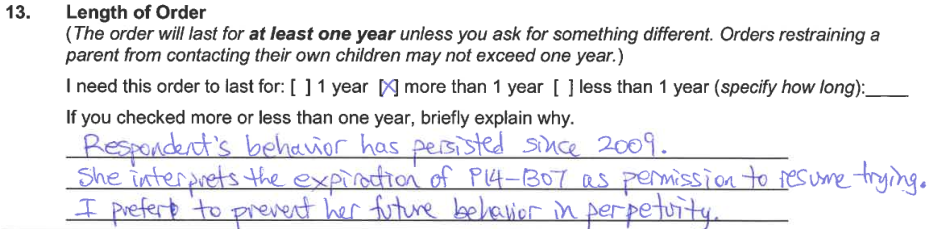
\includegraphics[width=.9\linewidth]{./pic/dearCousin_20220919_153711.png}
\begin{itemize}
\item 是的,我以为保护令的期限到了便是过期了,我便可以retry 恢复男女朋友关系了。。。
\item 听证会上,我向法官陈述了,我是国际留学生,对美国社会法律并不了解;
\end{itemize}
\section{最近的行为}
\label{sec-1-3}

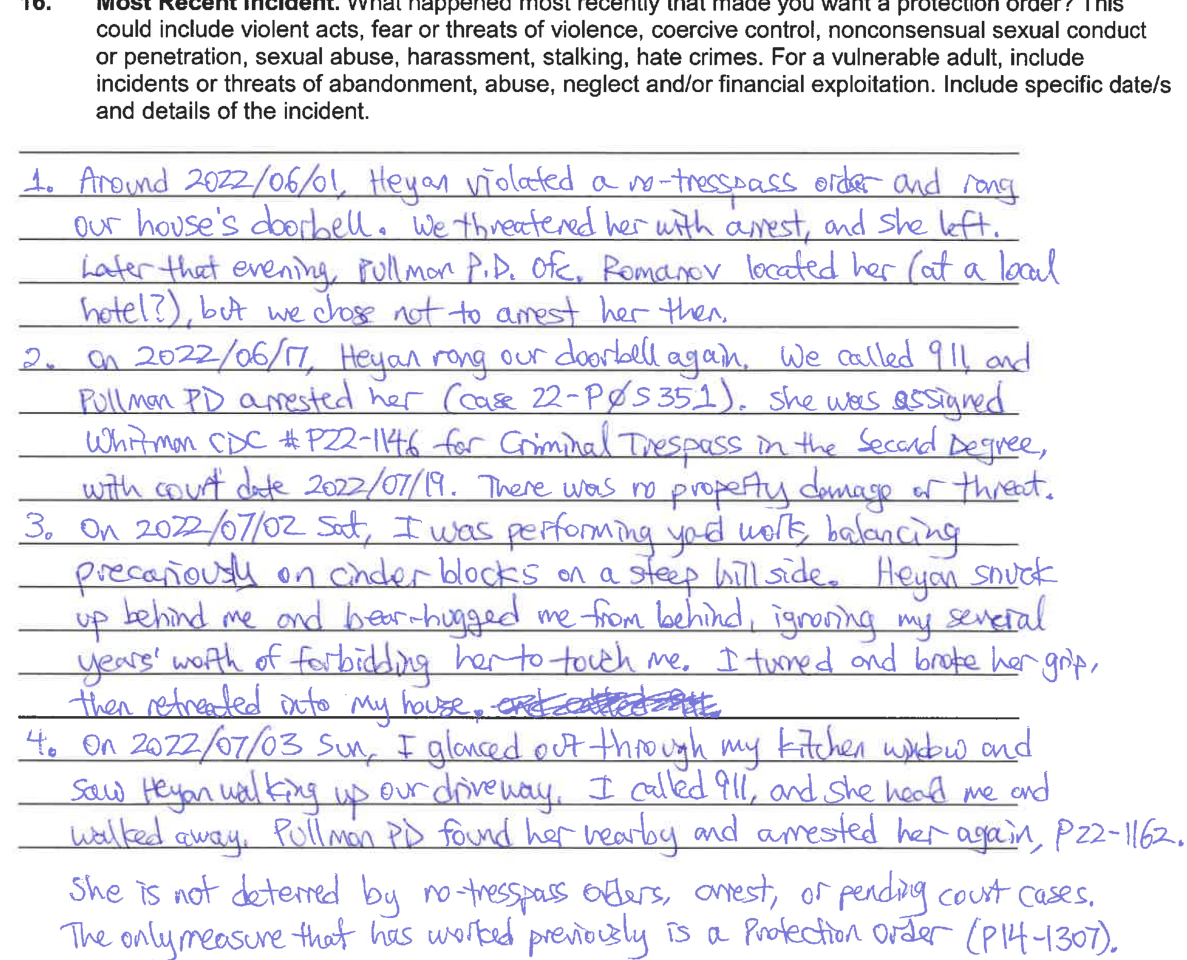
\includegraphics[width=.9\linewidth]{./pic/dearCousin_20220919_153946.png}
\section{以前的行为}
\label{sec-1-4}

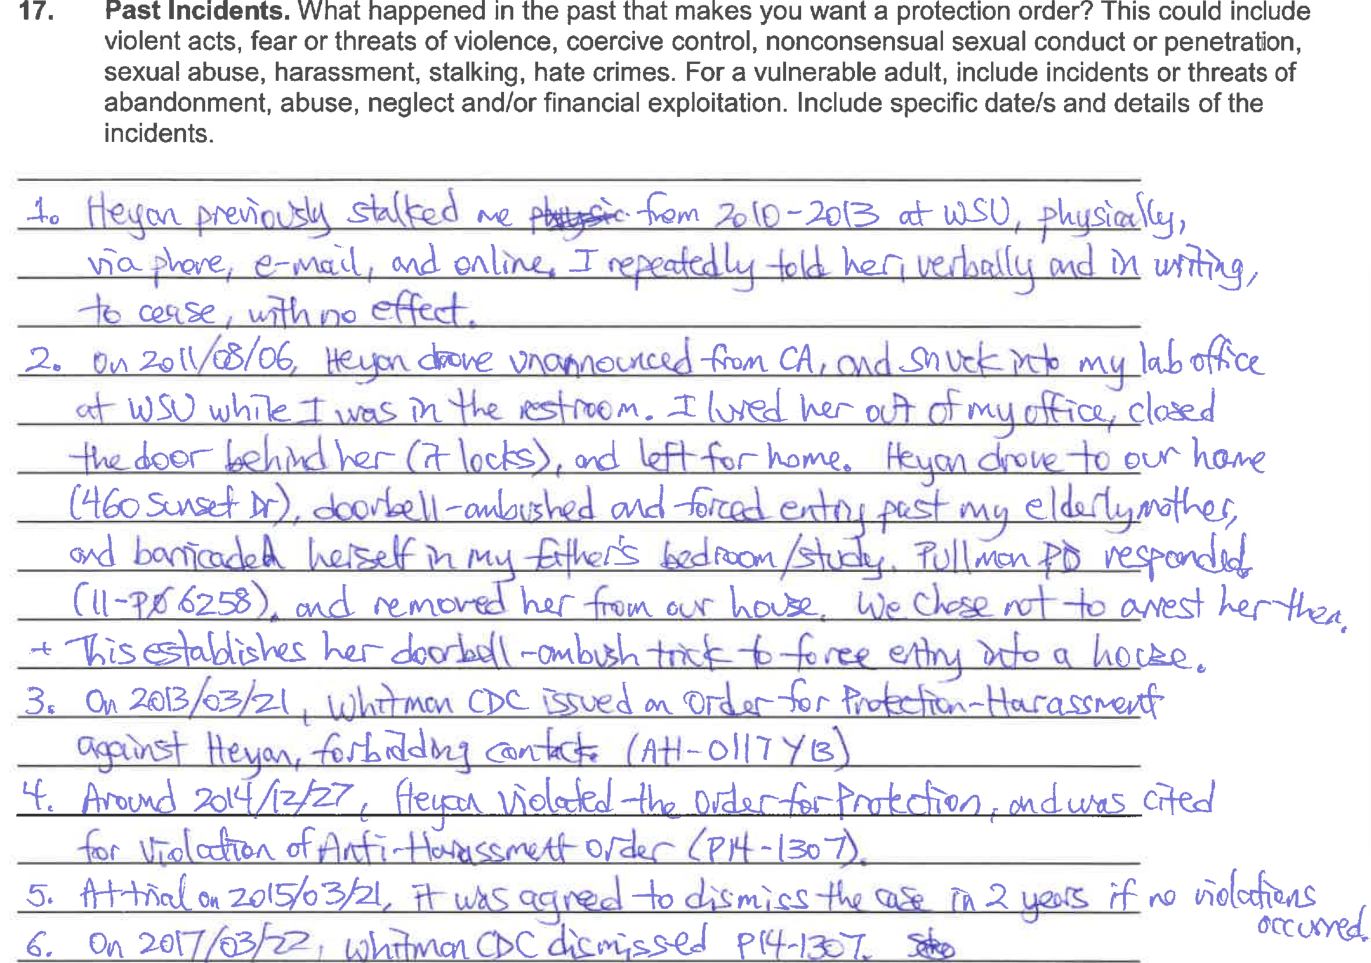
\includegraphics[width=.9\linewidth]{./pic/dearCousin_20220919_154045.png}

\chapter{个人的认知层面的问题  }
\label{sec-2}
\begin{itemize}
\item 法律是有期限的:所有的限制令都有过期的期限
\end{itemize}
\chapter{保护令下达(被小地方的法官一羊判便判成了一辈子--至2099呆槑槑槑槑 呵呵)后}
\label{sec-3}
\begin{itemize}
\item If you do not go to court, the judge can make the restraining order without hearing your side of the story. And the order can last up to 5 years.别人也就最多五年,他一弄就弄成了一辈子\url{https://www.courts.ca.gov/1279.htm?rdeLocaleAttr=en}
\item 原令保护令者,可是撒销保护令: The adverse party can file a Motion to Dissolve the protection order, and the court might schedule a hearing on the motion. The applicant can appear at the hearing to oppose the adverse party’s motion. If the Motion to Dissolve is granted after a hearing, the protection order will become immediately void and unenforceable.
\item 我可以appeal反保护令: The adverse party can file a Motion to Modify the protection order, and the court might schedule a hearing on the motion.
\item If an extended protection order is issued, the adverse party can file an appeal to the district court, and the district court might affirm, modify, or vacate the order. The extended protection order remains in effect during any appeal, unless the court orders otherwise.
\end{itemize}
\section{Appeal: \url{https://www.civillawselfhelpcenter.org/self-help/harassment-protection/modifying-dissolving-or-appealing-a-protection-order}}
\label{sec-3-1}
\begin{itemize}
\item What is an “appeal,” and how would I file one?
\begin{itemize}
\item If the court issues an extended order for protection, the adverse party can file an appeal to the district court. (There is no appeal allowed if the court denies an application to extend a protection order, only if the court grants the extension.) The district court will typically not hear new evidence on an appeal. The court will review the documentation and other information that was presented to the justice court in order to decide whether the justice of the peace made any error of law in granting the extended protection order.
\end{itemize}
\item The district court can affirm, modify, or vacate the justice court’s order. (In other words, the district court can keep the order in place, change it in some way, or do away with it completely.)
\item TIP!  If the hearing on the extended protection order you're appealing was recorded, you must order a copy of the hearing transcript from the court reporter and deposit \$100 with the court (unless some greater amount was ordered).  (JCRCP 74(b).)  If the hearing wasn't recorded, you must fill out and file the Statement of Evidence or Proceedings form below.
\end{itemize}

\chapter{Statements}
\label{sec-4}
\begin{itemize}
\item 现在的问题是我需要把文件也传给表哥吗?可是我只有一两天的时间[不用再担心这个问题,该发出去的邮件,该寄出去的材料全都寄出去了,最慢也三天之内可以到达了,不用担心]
\end{itemize}
-另外,法庭上还有哪些文件是需要我复制或是转达的吗{暂时也不骼担心这个问题,先把明天傍晚5点前需要上交的材料准备好,交上去,并同步发送给亲爱的表哥就可以了}
-我是否需要立即写封邮件问一下相关的工作人员{已经打电话问好了,就不要再担心了}
\chapter{oncline resources/ concepts diferences}
\label{sec-5}
\section{harassment vs Stalking}
\label{sec-5-1}
-槑槑呵呵)后
\chapter{Statements}
\label{sec-6}
\begin{itemize}
\item 现在的问题是我需要把文件也传给表哥吗?可是我只有一两天的时间[不用再担心这个问题,该发出去的邮件,该寄出去的材料全都寄出去了,最慢也三天之内可以到达了,不用担心]
\end{itemize}
-另外,法庭上还有哪些文件是需要我复制或是转达的吗{暂时也不骼担心这个问题,先把明天傍晚5点前需要上交的材料准备好,交上去,并同步发送给亲爱的表哥就可以了}
-我是否需要立即写封邮件问一下相关的工作人员{已经打电话问好了,就不要再担心了}
\chapter{oncline resources/ concepts diferences}
\label{sec-7}
\section{harassment vs Stalking}
\label{sec-7-1}
-“Harassment” occurs when:
\begin{itemize}
\item The adverse party threatens to harm another person in the future, damages another person’s property, confines or restrains another person, or does any act intended to substantially harm another person’s physical or mental health or safety; AND
\item The adverse party’s words or conduct causes the applicant to reasonably fear that the threats will be carried out.  (NRS 200.571.)
\item “Stalking” occurs when: 
\begin{itemize}
\item The adverse party engages in a course of conduct that would cause a reasonable person to feel terrorized, frightened, intimidated, or harassed or fearful for the immediate safety of a family or household member, AND
\end{itemize}
\end{itemize}
The applicant actually feels terrorized, frightened, or intimidated or fearful for the immediate safety of a family or household member.  (NRS 200.575(1).)

\chapter{写给偶们亲爱的表哥的情书}
\label{sec-8}
\begin{minted}[fontsize=\scriptsize,linenos=false]{text}
亲爱的表哥,
我总是忍不住想要给亲爱的表哥写点儿什么
我总是忍不住想要写给亲爱的表哥的冲动
要怎么组织自己的小脑袋瓜里的思路才能够
在亲爱的表哥面前更好在表达自己呢?
\end{minted}

\begin{itemize}
\item 下面是长周末,回家看表哥的时候写的
\begin{minted}[fontsize=\scriptsize,linenos=false]{text}
亲爱的表哥
这次回来
我终于找到了可是使用学校里帮助免费提供的无线网络
并且这次回来图书馆是开放的

不知道是不是前几天长途开车还没有缓过颈来
今天上午的脑袋还是昏昏的
还是说早上的咖啡里加得糖太多了犯昏呢?
于是乎,我再次坐进梦魅以求的图书馆里
做的事件是给亲爱的表哥写情书

每次回来
能够看见亲爱的表哥
我都总是狠开心
可是这次回来好几天了
我却还没能找到合适的机会看见亲爱的表哥

我知道舅舅和亲爱的表哥都是为我负责
所以才当年会早早地捶打911
无奈你的活宝妹早已是情根深种
心里面长了草种了草,心有所爱所庞
再来拔草
是舅舅和表哥用几十匹马、几十张火车皮来拉也拔不掉的

亲爱的表哥
10年底11年那时幼稚的自己
心心清清楚楚、明明白白地知道自己喜欢表哥
心里明白认定表哥
可是涉世不深,世俗里的障碍
让我固执地以为只要自己假装从来就不喜欢表哥
只要自己可以假装去爱上其它的人
只要自己能够按照世俗的标准
找个长相学历相配的人
便可以寐心地过完世俗标准下的一生

我以为我可以假装好一阵子
我以为我可以欺骗全世界
我以为我可以让所有的人都知道
我从来不曾爱过这样一位表哥
却原来我只假装得了一阵子
我以为我可以瞒天过海欺骗全世界
却原来我只是欺骗了我自己
浪费和虚度的从来都是自己的青春和光阴
我假装得了一时却假装不完一世

喜欢表哥
不是因为舅舅,不是因为任何感恩
情感中没有家庭轮理亲情关系上的感恩可言
更多也更应该是一个人内心情感的真正需求与向往
我喜欢表哥,不因为舅舅
喜欢表哥是因为,亲爱的表哥待我好
我曾被亲爱的表哥待我的好
真真切切、惊心动魂地感动过
感动到当时的自己就能清楚地认定
我遇见了对的人
这是我想要的幸福
我想要余生都被亲爱的表哥
温柔对待,时常宠爱,宠在心头掌心
亲爱的表哥,你看
你的这个妹妹从来都是把情感看得最重
把亲爱的表哥看得最重

曾经沧海难为水
除却巫山不是云
这两句话14个字成为我心口永远的痛
亲爱的表哥
我不止一次地问过你
你的心里是否留有别人的眼泪?
为什么你就一定接受不了你的这个活宝妹呢?
还是说,你只是简单地希望你的这个活宝妹
能够生活在大城市,能够物质上生活得相对好一点儿?

可是你的活宝妹从来都不是靠物质来活着的人呀
1997年当我第一次遇见舅舅的时候
2007年当我来到美国后再次找到舅舅的时候
真正能够捆绑和牵挂住人的从来都是情
是幼稚少女时代心有郁结时候的鼓励解脱
是心里有所向往便想要努力踏入这片向往的国度土地的愿望
你的妹妹从来不是靠物质活着的人
你的妹妹更多的是听从她自己内心的声音活着
可是亲爱的表哥
那场告别、那场遇见
亲爱的表哥与我能够走到一起,但是佳缘是天作之合
可是亲爱的表哥如果一再拒绝我,那你的妹妹我便成了在劫难逃
你的妹妹今生也无法逃过这场爱情的劫难
表哥,你一再拒绝,要你这个妹妹后半生怎么过?
终究还是只能导致这个妹妹后半生残破残缺不全的人生

我能够想到的两种原因,我个人更愿意去相信前者
人的情感难以理解却也最为强求不得
我无法强求亲爱的表哥寐心地娶我
但借由我自己的经历换位思考
希望亲爱的表哥即便如我所猜测般心有所属又求而不得
希望已经回到故乡、能够生活在亲人环绕中的表哥
在父母兄弟亲人的陪伴中能够渐渐放宽自己的标准
希望亲爱的表哥能够遇见自己喜欢的女孩子
或是亲爱的表哥能够与生活妥协、学会接纳你的活宝妹

问世间情为何物
只叫人生死相许
我的后半生最想要同亲爱的表哥生活在一起
可是生活的风浪不知道会将我(们)打向何方
即便亲爱的表哥一时半会儿近年月或是近一两年还不能接纳我
我也希望在不久的将来
亲爱的表哥能够遇见自己的幸福或是能够接纳我
任何时候,能够看见亲爱的表哥生活得幸福
都是我这辈子最快乐的事
虽然我自己想要的幸福,是与亲爱的表哥在一起

亲爱的表哥
这次走后,我还会经常回来
访寻亲爱的表哥、我们的足迹曾经遍历过的地方
哪天亲爱的表哥改变主意了
肯求亲爱的表哥一定第一时间告诉我
这辈子能够嫁给亲爱的表哥
对我来说,任何时候都不晚

自己寻找来到美国
能够遇见亲爱的表哥
对我来说,即便是情感里的在劫难逃
却也是生命的礼遇,我狠感激
要不然,生活就是一串口枯井,了无生趣
等我老了,若是还没能嫁给表哥
我就回来亲爱的表哥所在这个城镇
在亲爱的表哥家的对面或是不远处
买个小房子
每天能够看见亲爱的表哥从我的窗前经过
都会成为我每天最大的点缀与快乐
谢谢亲爱的表哥!今生能够遇见亲爱的表哥
是我最幸福快乐和感激的事
且行且珍惜
愿我们很快能够执子之手,携手到老!
\end{minted}
\end{itemize}

\chapter{LOVE MY DEAR COUSIN: looking for PROFESSIONAL help form attorneys in related fields}
\label{sec-9}
Hi, 

I am facing \textbf{two different charges from Whitman
County Pullman WA}. 

The charges are: 
\begin{itemize}
\item 9A.36.041.2: ASSAULT 4TH DEGREE
\item 9A.52.080: CRIMINAL TRESPASS-2ND DEGREE
\end{itemize}

I don't have any history with ASSAULT charges, and all the histories
of TRESPASS related were expired on 3/21/2017. 

I will be meeting the court judge soon within 2 - 3 weeks, and I am
looking for prefessional help to assist me though out the court dates and possibly
later trial. 

Please write to me \textbf{blue\_water\_000@hotmail.com}, if you are interested
and elligible for attorneys in \textbf{Whitman county, WA}, and please provide with your
quote as well. 

thanks. I look forward to hearing from you. 
% Emacs 27.1 (Org mode 8.2.7c)
\end{document}